Нехай між особинами є внутрішньовидова боротьба, що додає додаткове джерело загибелі.\\
Отже смертність: - природна:  $-\sigma x$;\\
\hspace*{4.01cm}- внутрішньовидова боротьба: $- \mu x^2$\\
Тоді швидкість народжуваності:$S = \gamma x$.\\
Швидкість смертності:  $ S = - \sigma x - \mu x^2$.\\
$$
\frac{dx}{dt}  = \gamma -  \sigma x - \mu x^2 = \underbrace{(\gamma - \sigma)}[=a] - \mu x^2
$$

\begin{center}
    \fbox{$ \frac{dx}{dt} = ax - \mu x^2 $} - закон Ферхюльста.
\end{center}
Нехай $a > 0$ (народжуваність > смертність).  Зауважимо, що $ax - \mu x^2 = x ( a - \mu x)$.

Проаналізувавши праву частину, бачимо, що:\\
$
\dfrac{dx}{dt} > 0 (\uparrow) \text{ при } x \in (0, \dfrac{a}{\mu} )
$\\
$
\dfrac{dx}{dt} < 0 (\downarrow) \text{ при } x \in (- \infty, 0) \cup ( \dfrac{a}{\mu},  +\infty)
$\\
$
\dfrac{dx}{dt} = 0 \text{ при } x = 0 \lor x = \dfrac{a}{\mu}
$\\


\begin{center} 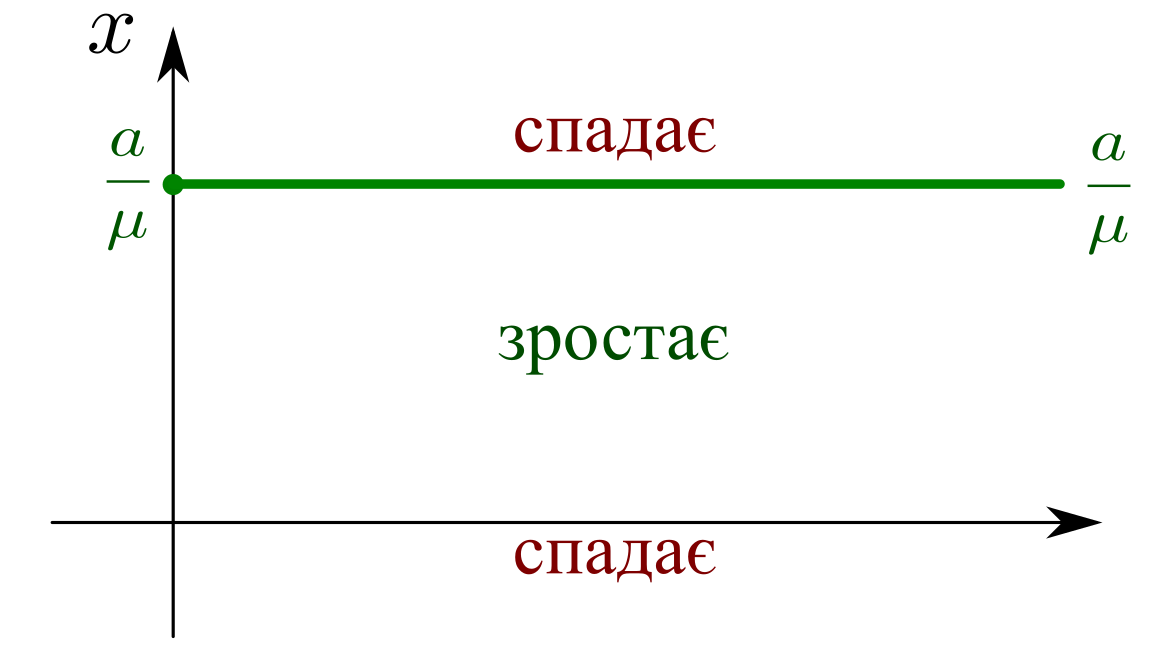
\includegraphics[scale=0.3]{assets/lectures_recent-e4b7cd02.png} \end{center}


Розв'яжемо рівняння: $ \dfrac{dx}{dt} = ax - \mu x^2 $ - рівняння Бернуллі.\\
$x = u\cdot v $\\
$u'v + v'u - auv = - \mu u^2 v^2 $\\
$u'v + u(v' - av) = - \mu u^2 v^2 $\\
$v' = av$\\
$ \dfrac{dv}{v} = adt \Longrightarrow v = e^{at}$\\
$u' =- \mu u^2 v$\\
$ \dfrac{du}{u^2} = - \mu e^{at}dt $\\
$- \dfrac{1}{u} = -\dfrac{ \mu}{a}e^{at} - C$\\
$ u = \dfrac{1}{ \frac{u}{a} e^{at} +c } = \dfrac{a}{ \mu e^{at} + aC} \Longrightarrow x = uv = \dfrac{a e^{at}}{ \mu e^{at} + aC  }  =  \dfrac{a}{ \mu  + aCe^{-at}}  $\\
$
\text{Отримали загальний розв'язок: } \left[ \begin{gathered}
 x= \frac{a}{ \mu  + aCe^{-at}}\\
 x = 0
\end{gathered} \right.
$\\


Знайдемо довільний розв'язок з.К. $x(t_0) = x_0:$
$$
x_0 = \frac{a}{\mu + aCe^{-at_0}}
$$
$$
\mu + aC\cdot e^{-at_0} = \frac{a}{x_0}
$$
$$
C = \frac{\left( \frac{a}{x_0} - \mu  \right)\cdot e^{at_0} }{a} = \frac{a - \mu x_0}{ax_0}\cdot e^{at_0} \Longrightarrow
$$
$$
\Longrightarrow x(t) = \frac{a}{ \mu + \frac{a - \mu x_0}{x_0} \cdot e^{a(t_0 - t)} } = \frac{ax_0}{ \mu x_0 - (a - \mu x_0 ) \cdot e^{a(t_0-t)}}
$$
Розв'язок $ \varphi (t) = \frac{a}{\mu} \quad \exists $  на $[0, + \infty)$.\\
Перевіримо другу умову стійкості. \\
Візьмемо $ \left| x - \frac{a}{\mu} \right| = \left| \frac{\mu x_0 - a}{\mu}  \right| < \delta $ і розглянемо:
$$
\left| x(t) - \varphi(t) \right| = \left| \frac{ax_0}{\mu x_0 - (a - \mu x_0) \cdot e^{a (t_0 - t)}}  - \frac{a}{ \mu}  \right| =
$$
$$
= \left| \frac{a\mu x_0 - a\mu x_0 + a (a - \mu x_0 )\cdot e^{a(t_0 - t)}}{\mu (\mu x_0 - (a- \mu x_0)\cdot e^{a(t_0 -t)})}  \right| = \frac{a (a - \mu x_0)\cdot e^{a (t_0 - t)}}{ \mu^2 x_0 - \mu (a- \mu x_0) \cdot e^{a(t_0 - t)}} \xrightarrow[t\to +\infty]{} 0
$$

Таким чином, розв'язок $\varphi(t) = \frac{a}{\mu}$ - асимптотично стійкий.
\begin{center} 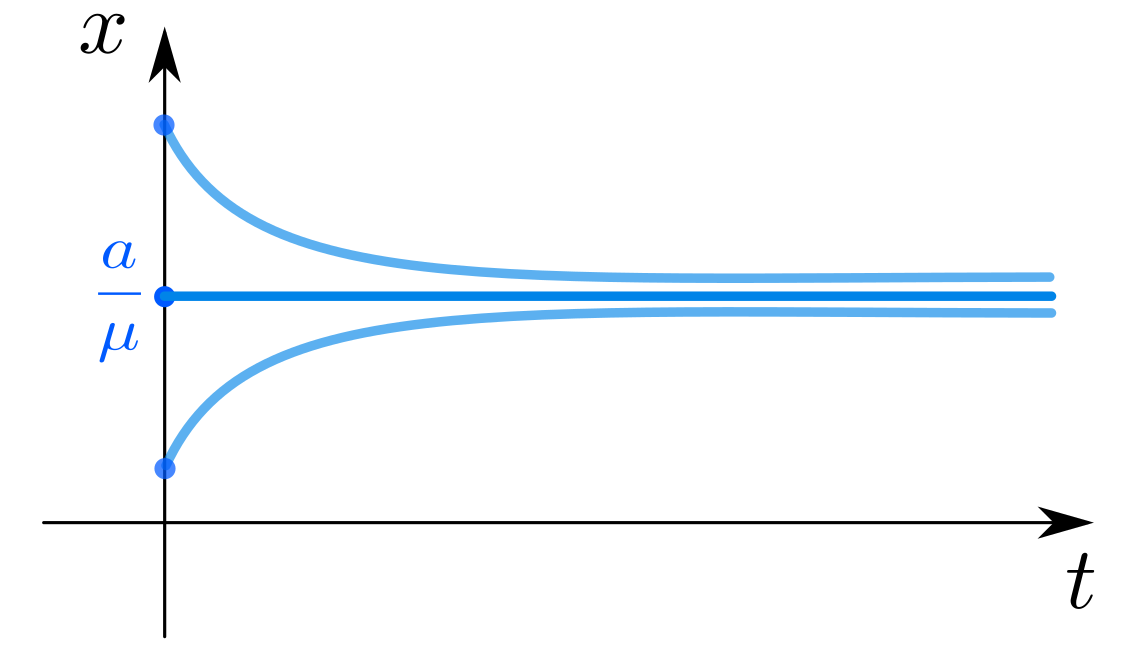
\includegraphics[scale=0.3]{assets/lectures_recent-0b98e3f0.png} \end{center}
\begin{remark}
    1. Аналогічно можна показати, що $\varphi (t) = 0$ - нестійкий. Таким чином, внутрішньовидова боротба виступає ''природнім стабілізатором'' моделі одновимірної популяції. \\
    На відміну від моделі Мальтуса, де у випадку $ a > 0$ маємо нестійкість і нескінчений ріст популяції, в моделі Ферхюльста розв'язки стабілізуються в околі стлого розв'язку $\varphi(t) = \frac{a}{\mu}.$ Відзначимо також, що чим меньше значення $\mu$, тим швидше зростає чисельність особин.
\end{remark}

\begin{remark}
    2. При $ a\leq 0$ (смертність $\geq$  народжуваність) легко встановити, що $ x=0 $ - асимптотично стійкий розв'язок.
\end{remark}

\subsection{Класифікація фазових портретів в околі положень рівноваги ЛОС 2-го порядку.}

\begin{defo}
    Положенням рівноваги нормальної системи диф. рівнянь:
    $$
    \begin{dcases}
        \dot{x_1} = f_1(x_1, ..., x_n)\\
        \qquad \quad \cdots\\
        \dot{x_n} = f_n(x_1, ..., x_n)
    \end{dcases}
    $$
    називається т. $\overline{x} = (x_1, ... , x_n)$ така, що:
    $$
    f_1 (\overline{x}) = f_2(\overline{x}) = \cdots = f_n(\overline{x}) =0
    $$
\end{defo}
Розглянемо ЛОС (1):$ \begin{cases}
    \dot{x} = ax + by\\
    \dot{y} = cx + dy
\end{cases}$, де $a,b,c,d \in \mathbb{R} \quad A = \begin{bmatrix}
 a & b\\
 c & d
\end{bmatrix}$.\\
Нехай $\det A \neq 0$. Тоді єдине положення рівноваги системи (1) - це т. (0,0).
\begin{defo}
    Фазовою траєкторією ЛОС (1) називається проекція її інтегральних кривих на площину $X0Y$. Зображення фазових траєкторій на площині $X0Y$ називають фазовим портретом.
\end{defo}
\textbf{Завдання.} Дослідити фазовий портрет ЛОС (1) в околі точки (0, 0), яка є її положенням рівноваги.\\

Виявляється, що фазовий портрет ЛОС (1) в околі т. (0,0) повністю визначається власними числами матриці $A$. Нехай $J(A)$ - ЖНФ матриці $A$; $H$ - матриця переходу.\\

1. Нехай $\lambda_1 , \lambda_22 \in \mathbb{R} \quad \lambda_1 \neq \lambda_2 \quad \lambda_1 \cdot \lambda_2 > 0.$\\ Для зручності здійснимо в системі (1):
$$
\begin{bmatrix}
 \dot{x}\\
 \dot{y}
\end{bmatrix} = A \begin{bmatrix}
 x \\
 y
\end{bmatrix} \text{ заміну: } \begin{bmatrix}
 x\\
 y
\end{bmatrix} = H \begin{bmatrix}
 u, h
\end{bmatrix},
$$
де $\begin{bmatrix}
 u \\
 v
\end{bmatrix}$ - нова невідома вектор-функція.
$$
H \cdot \begin{bmatrix}
 \dot{u}\\
 \dot{v}
\end{bmatrix} = A \cdot H \cdot \begin{bmatrix}
 u \\
 v
\end{bmatrix} \qquad \text{домножимо зліва на } H^{-1}
$$
$$
H^{-1} \cdot H \begin{bmatrix}
\dot{u}\\
\dot{v}
\end{bmatrix}  =H^{-1} \cdot A \cdot H \cdot \begin{bmatrix}
 u \\
 v
\end{bmatrix}
$$
$$
\begin{bmatrix}
\dot{u}\\
\dot{v}
\end{bmatrix}  =J(A) \cdot \begin{bmatrix}
 u \\
 v
\end{bmatrix}
$$
Таким чином, ми перейшли до Жарданового базису.\\
Маємо: $ \begin{bmatrix}
\dot{u}\\
\dot{v}
\end{bmatrix} = \begin{bmatrix}
 \lambda_1 & 0 \\
 0 & \lambda_2
\end{bmatrix} \begin{bmatrix}
 u \\
 v
\end{bmatrix}$
